
“类型和对象基本概念表”列出了类型和对象的基本概念。

“范围、迭代器和算法概念表”列出了范围、视图、迭代器和算法的概念。

辅助概念表列出的概念主要用作其他概念的构建块,通常不会让应用程序开发者直接使用。

\mySubsubsection{5.1.1}{头文件和命名空间}

标准概念在不同的头文件中定义:

\begin{itemize}
\item
头文件<concepts>中定义了许多基本概念,其中包括<ranges>和<iterator>。

\item
迭代器的概念在头文件<iterator>中定义。

\item
范围的概念在头文件<ranges>中定义。

\item
<compare>中定义了three\_way\_comparable的概念(几乎包含在所有其他头文件中)。

\item
uniform\_random\_bit\_generator在<random>中定义。
\end{itemize}

几乎所有的概念都定义在命名空间std中,唯一的例外是range概念,它定义在命名空间std::ranges中。

\begin{longtable}[c]{|l|l|}
\hline
\textbf{概念} &
\textbf{约束} \\ \hline
\endfirsthead
%
\endhead
%
\begin{tabular}[c]{@{}l@{}}integral\\ signed\_integral\\ unsigned\_integral\\ floating\_point\end{tabular} &
\begin{tabular}[c]{@{}l@{}}整型\\ 有符号整型\\ 无符号整型\\ 浮点类型\end{tabular} \\ \hline
\begin{tabular}[c]{@{}l@{}}movable\\ copyable\\ semiregular\\ regular\end{tabular} &
\begin{tabular}[c]{@{}l@{}}支持移动初始化/赋值和交换\\ 支持移动和复制初始化/赋值和交换\\ 支持默认初始化、复制、移动和交换\\ 支持默认初始化、复制、移动、交换和相等比较\end{tabular} \\ \hline
\begin{tabular}[c]{@{}l@{}}same\_as\\ convertible\_to\\ derived\_from\\ constructible\_from\\ assigneable\_from\\ swappable\_with\\ common\_with\\ common\_reference\_with\end{tabular} &
\begin{tabular}[c]{@{}l@{}}相同类型\\ 类型可转换为另一类型\\ 从另一类型派生的类型\\ 可从其他类型构造的类型\\ 可从另一类型赋值的类型\\ 类型可与其他类型交换\\ 两种类型有一个共同的类型\\ 两个类型有一个共同的引用类型\end{tabular} \\ \hline
\begin{tabular}[c]{@{}l@{}}equality\_comparable\\ equality\_comparable\_with\\ totally\_ordered\\ totally\_ordered\_with\\ three\_way\_comparable\\ three\_way\_comparable\_with\end{tabular} &
\begin{tabular}[c]{@{}l@{}}类型支持相等性检查\\ 可以检查两种类型是否相等\\ 类型支持严格的弱排序\\ 是否可以检查两种类型的严格弱排序\\ 可以应用所有比较运算符(包括运算符\textless{}=\textgreater{})\\ 可以使用所有比较操作符(包括 \textless{}=\textgreater{})\end{tabular} \\ \hline
\begin{tabular}[c]{@{}l@{}}invocable\\ regular\_invocable\\ predicate\\ relation\\ equivalence\_relation\\ strict\_weak\_order\\ uniform\_random\_bit\_generator\end{tabular} &
\begin{tabular}[c]{@{}l@{}}类型是指定参数的可调用对象\\ 类型是指定参数的可调用对象(无修改)\\ 类型是一个谓词(返回布尔值的可调用对象)\\ 可调用类型定义了两个类型之间的关系\\ 可调用类型定义了两个类型之间的相等关系\\ 可调用类型定义了两个类型之间的排序关系\\ 可调用类型可以用作随机数生成器\end{tabular} \\ \hline
\end{longtable}

\begin{center}
表5.1 类型和对象的基本概念
\end{center}

\begin{longtable}[c]{|l|l|}
\hline
\textbf{概念} &
\textbf{约束} \\ \hline
\endfirsthead
%
\endhead
%
\begin{tabular}[c]{@{}l@{}}default\_initializable\\ move\_constructible\\ copy\_constructible\\ destructible\\ swappable\\ weakly\_incrementables\\ incrementable\end{tabular} &
\begin{tabular}[c]{@{}l@{}}类型可默认初始化\\ 类型支持移动初始化\\ 类型支持复制初始化\\ 类型是可销毁\\类型可交换\\ 类型支持自增操作符\\ 类型支持保持相等的递增运算符\end{tabular} \\ \hline
\end{longtable}

\begin{center}
表5.2 辅助概念
\end{center}

\begin{longtable}[c]{|l|l|}
\hline
\textbf{概念} &
\textbf{约束} \\ \hline
\endfirsthead
%
\endhead
%
\begin{tabular}[c]{@{}l@{}}range\\ output\_range\\ input\_range\\ forward\_range\\ bidirectional\_range\\ random\_access\_range\\ contiguous\_range\\ sized\_range\\ common\_range\\ borrowed\_range\\ view\\ vieable\_range\end{tabular} &
\begin{tabular}[c]{@{}l@{}}类型是一个范围\\ 类型是要写入的范围\\ 类型是要读取的范围\\ 类型是一个可多次读取的范围\\ 类型是向前和向后读取的范围\\ 类型是一个支持在元素上跳跃的范围\\ 类型是在连续内存中包含元素的范围\\ 类型是一个大小支持范围\\ 类型是一系列迭代器和相同类型的哨兵\\ 类型是左值或借用的范围\\ 类型是视图\\ 类型或可以转换为视图\end{tabular} \\ \hline
\begin{tabular}[c]{@{}l@{}}indirectly\_writable\\ indirectly\_readable\\ indirectly\_movable\\ indirectly\_movable\_storable\\ indirectly\_copyable\\ indirectly\_copyable\_storable\\ indirectly\_swappable\\ indirectly\_comparable\end{tabular} &
\begin{tabular}[c]{@{}l@{}}类型可用于写入它所引用的位置\\ 类型可用于从其所引用的位置进行读取\\ 类型是指可移动的对象\\ 类型是指支持临时的可移动对象\\ 类型指的是可复制对象\\ 类型是指支持临时对象的可复制对象\\ 类型指的是可交换的对象\\ 类型指的是可比较的对象\end{tabular} \\ \hline
\begin{tabular}[c]{@{}l@{}}input\_output\_iterator\\ output\_iterator\\ input\_iterator\\ forward\_iterator\\ bidirectional\_iterator\\ random\_access\_iterator\\ contiguous\_interator\\ sentinel\_for\\ sized\_sentinel\_for\end{tabular} &
\begin{tabular}[c]{@{}l@{}}类型是一个迭代器\\ 类型是一个输出迭代器\\ 类型(至少)是输入迭代器\\ 类型(至少)是前向迭代器\\ 类型(至少)是一个双向迭代器\\ 类型(至少)是一个随机访问迭代器\\ 类型是指向连续内存中元素的迭代器\\ 类型可以用作迭代器类型的标记\\ 类型可以用作迭代器类型的哨点,距离计算的成本较低\end{tabular} \\ \hline
\begin{tabular}[c]{@{}l@{}}permutable\\ mergeable\\ sortable\end{tabular} &
\begin{tabular}[c]{@{}l@{}}类型(至少)是一个前向迭代器,可以对元素重新排序\\ 可以使用两种类型将排序后的元素合并为第三种类型\\ 类型是可排序的(根据比较和投影)\end{tabular} \\ \hline
\begin{tabular}[c]{@{}l@{}}indirectly\_unary\_invocable\\ indirectly\_regular\_unary\_invocable\\ indirect\_unary\_predicate\\ indirect\_binary\_predicate\\ indirect\_equivalence\_relation\\ indirect\_strict\_weak\_order\end{tabular} &
\begin{tabular}[c]{@{}l@{}}操作可以用迭代器的值类型调用\\ 无状态操作可以用迭代器的值类型调用\\ 一元谓词可以用迭代器的值类型调用\\ 二元谓词可以用两个迭代器的值类型调用\\ 谓词可用于检查传递的迭代器的两个值是否相等\\ 谓词可用于对传递的迭代器的两个值排序。\end{tabular} \\ \hline
\end{longtable}

\begin{center}
表5.3 范围、迭代器和算法的概念
\end{center}

\mySubsubsection{5.1.2}{标准概念的包含}

C++标准库提供的概念经过精心设计,以便在有意义时包含其他概念,其建立了一个相当复杂的包含图。图5.1显示了它的复杂程度。

\begin{center}
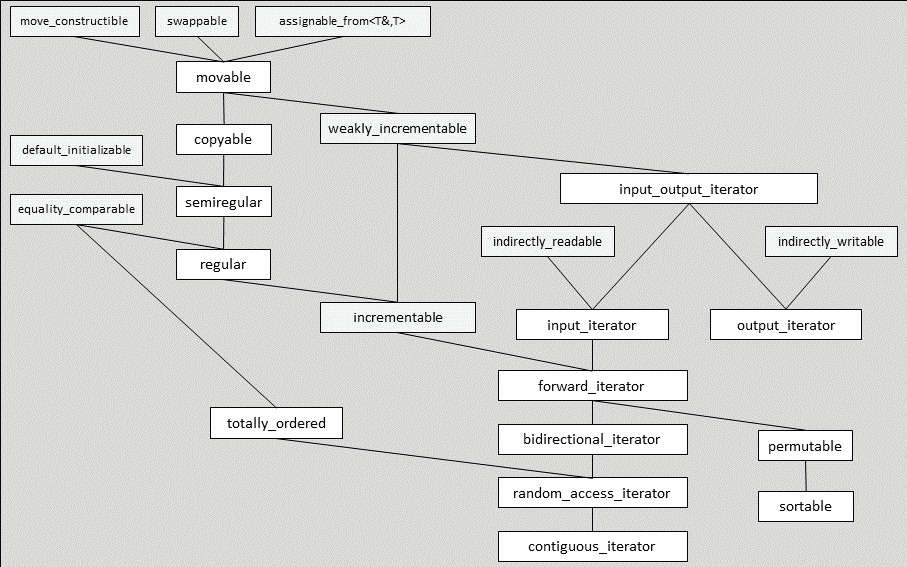
\includegraphics[width=1.\textwidth]{content/chapter5/images/1.png}\\
图5.1 C++标准概念的包含图(摘录)
\end{center}

出于这个原因,概念的描述列出了包含哪些其他关键概念。



